% Especificaciones del tamaño de letra, tamaño de hoja, márgenes, librerias, etc.
\documentclass[letterpaper]{article}
\usepackage[english]{babel}
\usepackage[utf8]{inputenc}
\usepackage[T1]{fontenc}
\usepackage{mathrsfs}
\usepackage{amsmath}
\usepackage{graphicx}
\usepackage[justification=centering]{caption}
\usepackage{subcaption}
\usepackage[hidelinks]{hyperref}
\usepackage{url}
\usepackage{amssymb}
\usepackage{float}
\usepackage[framed, numbered]{matlab-prettifier}
\usepackage{lipsum}
\usepackage{multicol}
\usepackage{fancyhdr}
%\usepackage[framed, numbered, autolinebreaks, useliterate]{mcode}
\usepackage[margin=1in]{geometry}
\usepackage{titlesec}
\titlelabel{\thetitle.\quad}
\titleformat*{\section}{\normalsize\centering}
\titleformat*{\subsection}{\normalsize\centering}
\renewcommand{\thesection}{\Roman{section}}
\renewcommand{\baselinestretch}{1.3}

\pagestyle{fancy}
\fancyhf{}
\rhead{C. A. VÁSQUEZ}
\lhead{ON COMPOSITE MATERIALS}
\rfoot{\thepage}

% Enlace Bibliografía
\usepackage{csquotes}
\usepackage[backend=biber, sorting=none]{biblatex}
\addbibresource{referencias.bib}

% Titulo, autores, fecha.
\title{\textbf{ON COMPOSITE MATERIALS AND THEIR FUTURE IN THE AEROSPACE INDUSTRY}}
\author{C. A. Vásquez\\
\footnotesize {\textit{UABC, Engineering Department, Mexicali, México}}\\
\footnotesize \texttt{a1155057@uabc.edu.mx}}
\date{}
% Inicio del documento
\begin{document}
\maketitle

\begin{abstract}
	The use of composite materials has given us the ability to build more lightweight and more fuel efficient aircraft. The possibilities these have given us are numerous, but in order to take full advantage of them we first need to understand them. We will discuss the characteristics and properties of these materials and how they are used today to make aircraft the most optimized it has ever been. Afterwards we will discuss the way new composite materials are being created and what the future holds for these.
\end{abstract}
	{\bf Keywords---} composite, aircraft, aerospace

\begin{multicols}{2}
	\section{INTRODUCTION}
	The overall purpose of this document is to discuss the nature of composite materials and talk to a certain extent about what they promise to the aerospace industry. Looking back at the now obsolete aircrafts from the past, they relied on a handful of materials that made them very heavy and very fuel inefficient. Nowadays, the aerospace industry is looking for alternative materials to reduce fuel consumption and make designs that are safer and better performers. These materials not only serve aerospace engineers, they also are very sought after by engineers in the automotive, infrastructure, military and space industry. The need of these materials has been increasing during the last four decades given that they offer great value despite of their cost to develop and manufacture them.

	Thanks to private companies such as Airbus and Boeing making efforts to incorporate composite into primary load carrying structures of large commercial transports and to certify their worthiness, is evident there is a significant value in the advancements made in understanding these structures. \supercite{nasa09}

	As a whole, this paper aims to (1) explain the basics of composite materials and why they are of interest in the industry, (2) the way composite materials are classified, (3) the way we quantize the failure of a material and the different theories used for each of them, (4) how these materials are being used in the present and (5) what we can expect from the advancements in material technology and what they can promise.
	\section{THE NATURE OF COMPOSITE MATERIALS}
	Composite materials have been used by organisms and early lifeforms as they have proved to be effective in what they do. The most prevalent example is wood. It's made from long cellulose fibers which are held by a substance called lignin. Lignin and cellulose together form a much stronger material. Other early examples are mud bricks, which are made of mud and straw, giving the whole mud brick resistance to stress under compression and tension.

	Composite materials are made by combining two or more materials, often ones that have very different properties. These materials work together in order to give the composites unique properties. Most composites are made of just two materials, one is the \textit{matrix} or \textit{binder}, which surrounds and binds together fibres or fragment of the other material, which is called the \textit{reinforcement}.\supercite{rsc} It's necesarry to make the following remark: in contrast to metallic alloys, each material retains its separate chemical, physical, and mechanical properties.
	\begin{figure}[H]
		\centering
		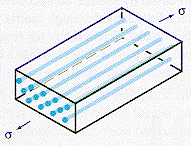
\includegraphics[width=0.5\textwidth]{mf.png}
		\caption{General layout of a composite material. Shown in blue are the fibers and the space in between is the matrix.}
	\end{figure}
	The biggest advantage of these materials is that, by choosing the right matrix and reinforcement, a new material can be made that meets the criteria for a specific application aswell as the right size and shape (composites are known to be very flexible when designing and can be moulded into complex shapes). The biggest disadvantage is cost as the raw materials needed to make the composite are often expensive, but the advantages make up for these drawbacks. As we will see, some composite materials can be strong and lightweight at the same time, which is convinient for modern aircraft.

	\section{THE BASIC PRINCIPLES}
	As discussed earlier, composite materials are made by two main components: the \textit{matrix}, a continuous component and the \textit{fiber} (also known as \textit{filler}), the discrete or discontinuous component. Given these two basic bulding blocks for composite materials, we have a classification depending on what type of material we use for either of them.
	\subsection*{CLASSIFICATION BASED ON MATRIX}
	There are different types of composites depending on the type of materials used in the matrix. These include: ceramic matrix composites (CMC), polymer matrix composites (PMC) and metal matrix composites (MMC) \supercite{owonubi19}
	Although it's difficult to give an exact description of the properties of these types of composites, at a simplistic level some obvious characteristic properties can be identified:
	
	\textbf{Metal Matrix Composites:} Mostly of medium to high density, they have good thermal stability and can be made corrosion-resistant by alloying. Metals have useful mechanical characteristics and it is moderately easy to shape and join.

	\textbf{Ceramic Matrix Composites:} Great thermal stability and are resistant to corrosion, abrasion and other forms of attack. They are very rigid but mostly brittle and can only be shaped with difficulty.
	
	\textbf{Polymer Matrix Composites:} Are of low density, they have a good chemical resistance but lack thermal stability. They have poor mechanical properties, but are easily fabricated and joined. Their resistance to environmental degradation is moderate. \supercite{altenbach04}

	The classifications given above are the main classes based on matrix but these have different subclasses that are shown in figure 3.

	\subsection*{CLASSIFICATION BASED ON REINFORCEMENT}
	The reinforcing phase provides the strength and stiffness. In most cases, the reinforcement is harder, stronger, and stiffer than the matrix, and is usually a fiber or a particulate.

	\textbf{Fiber Reinforcement:} A fiber has a length that is much greater than its diameter. The length-to-diameter ratio ($d/l$) is known as the \textit{aspect ratio} and can vary greatly. Continuous fibers have long aspect ratios and normally have a preferred orientation, while dicontinuous fibers have short aspect ratios and generally a random orientation.
	Examples of continuous reinforcements include unidirectional, woven cloth, and helical winding (fig. 2a), while examples of discontinuous reinforcements are chopped fibers and random mat (fig. 2b)
	
	\textbf{Particulate Reinforcemente:} They have dimensions that are approximately equal in all directions. They may be spherical, platelets, or any other regular or irregular geometry. Particulate reinforcement tend to be much weaker and less stiff than continuous-fiber composites, but they are usually less expensive.\supercite{campbell10}

	After explaining the overall characteristics and general description of each type of composite material, figure 3 shows a chart where the classification of composite materials is (a) based on matrix materials and (b) based on reinforcement materials.
\end{multicols}

\begin{figure}[H]
	\centering
	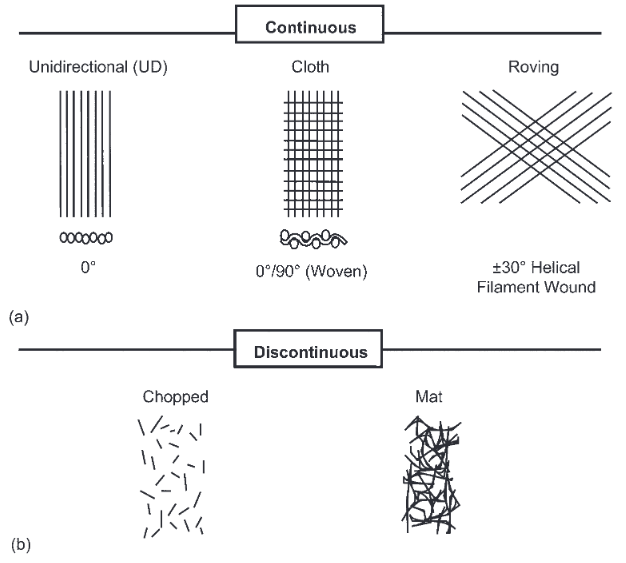
\includegraphics[width=0.9\textwidth]{reinforcements.png}
	\caption{Examples of different types of fiber reinforcements.}
\end{figure}

\begin{figure}[H]
	\centering
	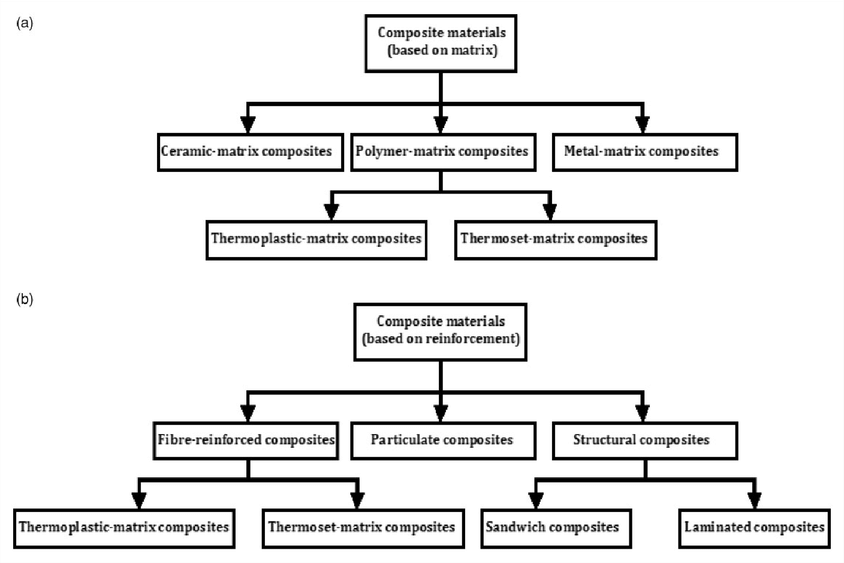
\includegraphics[width=\textwidth]{class.png}
	\caption{Chart of the different classifications of composite materials. Obtained from \autocite{idowu15}}
\end{figure}
\begin{multicols}{2}
	\textbf{Structural Composites:} In this category the design is taking advantage of the structure of the material and combines it in a way that stress is properly distributed and produces less strain. Usually a fiber-reinforced material is used to make the different layers needed in order to make the structural composite. In a way, these materials are a subcategory of the fiber-reinforced composites. \textbf{Laminated composites} or \textbf{crossplied laminates} are the most common structural composites, in which the fabricator "lays up" a sequence of unidirectional reinforced "plies" (plural for "ply") as indicated in figure 4. Each ply is tipicaly a thin sheet of collimated fibers impregnated with an uncured epoxy or other thermosetting polymer matrix material. \supercite{roylance00}
	
	On the other hand, a \textbf{sandwich structure} is a fabricated material which consists of two thin, stiff facing sheets joined to either side of a low dnsity core material or structure. The separation of the facings by a lightweight core acts to significantly increase the second moment of area (and hence the bending stiffness) of the material cross-section with only a small increase in weight. This is known as the \textit{sandwich effect}\supercite{sandcore}, illustrated in figure 5.
	\begin{figure}[H]
		\centering
		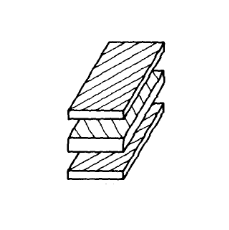
\includegraphics[width=0.3\textwidth]{laminate.png}
		\caption{A 3-ply symmetric laminate. Obtained from \autocite{roylance00}}
	\end{figure}

	\begin{figure}[H]
		\centering
		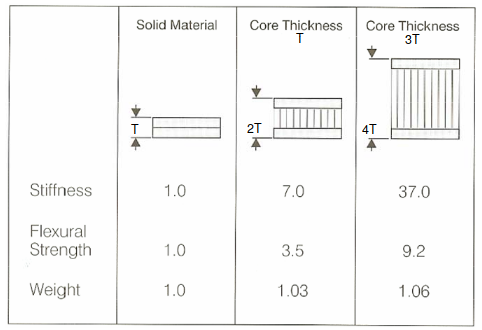
\includegraphics[width=0.5\textwidth]{sandwicheffect.png}
		\caption{Illustration of the \textit{sadnwich effect}. It can be seen that it is possible to realise significant increases in bending stiffness and strength for minimal increases in weight compared to a single skin structure (i.e. laminates).\supercite{sandcore}}
	\end{figure}
	\subsection*{BASED ON THE COMPOSITION}
	Althought we've talked about the classifications of materials based on matrices and reinforcements, there's another way of grouping them, which consist in the nature of their properties and how they are conserved (or not conserved) throughout the material as a whole.
	
	\textbf{Isotropic Materials:} These materials have the same material properties in all directions, and normal loads create only normal strains. A material is isotropic if the properties are independent of direction within the material.

	\textbf{Anisotropic Materials:} Anisotropic materials have different material properties in all directions at a point in the body. There are no material planes of symmetry, and normal loads create both normal and shear strains.\supercite{campbell10}

	\textbf{Orthotropic Materials:} Are a subset of anisotropic materials, where the shear stresses are decoupled from normal stresses, exhibiting different stiffnesses in three orthogonal directions. \supercite{li14} In other words, the properties these materials have are different in three mutually perpendicular directions. They have three mutually perpendicular axes of symmetry, and a load applied parallel to these axes produce both normal and shear strains.
	
	\section{FAILURE}
	When a load is applied on a material, it will produce a certain strain and stress on it. If the stress produced in the body due to the application of the load is beyond the elastic limit, permanent deformation occurs. Whenever this occurs, the body is said to have \textit{failed}. This should make clear that when a material fails it does not mean ti has ruptured.
	Being able to determine when a material will fail, break or fissure has been a long time question that has multiple answers. It depends on wether the material is brittle or ductile, as they have different properties that are obvious when we see their stress-strain graphs side by side, as seen in figure 4. Identifying and finding when the material in question will fail is absolutely necessary if we want to design a product that accomplishes all the security requirements.
	
	\begin{figure}[H]
		\centering
		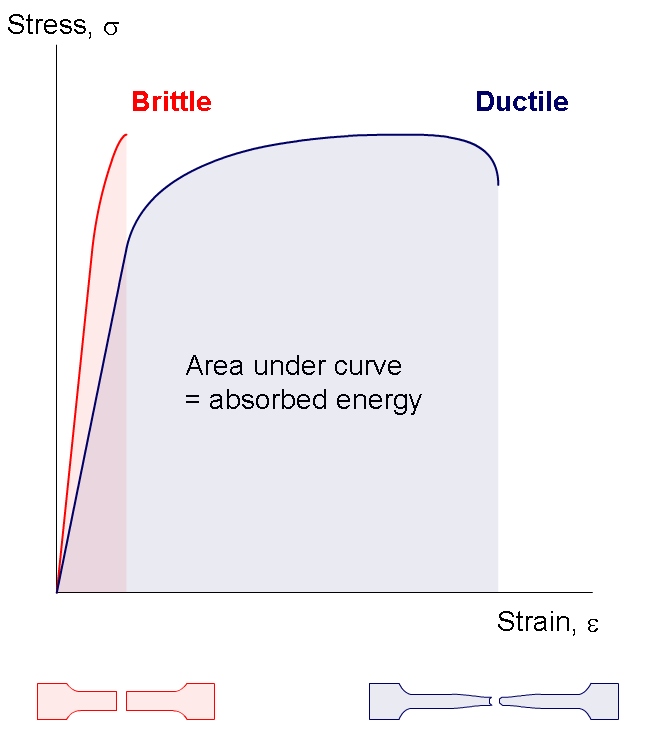
\includegraphics[width=0.4\textwidth]{stressstrain.png}
		\caption{Brittle materials fracture at low strains and absorb little energy while ductile materials fail after significant plastic strain and absorb more energy.}
	\end{figure}
	Either type of material we choose, there have been several theories developed, which are classified into three main groups.\supercite{rajanish13}

	\subsection*{LIMIT OR NONINTERACTIVE THEORIES}
	\begin{itemize}
		\item Maximum Stress Theory: There are several failure theories based on the maximum stress, and it all depends on the type of material is being analyzed. On of the most used is the \textbf{maximum principal stress theory}, also known as \textit{Rankine's theory}. According to this theory, the failure of the materialwill occure when the maximum principal tensile stress ($\sigma_1$) in the complex system reaches the value of the maximum stress at the elastic limit in simple tension or the minimum principal stress (i.e., the maximum principal compressive stress) reaches the value of the maximum stress at the elastic limit in simple compression.\supercite{bansal09}

			Let, in a complex three dimensional stress system,

			$\sigma_1$, $\sigma_2$ and $\sigma_3$ = principal stresses at a point in three perpendicular directions. The stresses $\sigma_1$ and $\sigma_2$ are tensile and $\sigma_3$ is compressive. Also $\sigma_1 > \sigma_2$.

			$\sigma_t$ = tensile stress at elastic limit in simple tension.

			$\sigma_c$ = compressive stress at elastic limit in simple tension.

			According to the stabilished before, the failure will take place if:

			$\sigma_1 \geq \sigma_t$ in simple tension or $\mid \sigma_3 \mid \ \geq \sigma_c$ in simple compression.

			This is the simplest and oldest theory of failure. If the maximum principal stress ($\sigma_1$) is the design criterion, then maximum principal stress must not exceed the permissible stress ($\sigma_t$) for the given material.

		\item Maximum Strain Theory: Similar to the maximum stress theory, the maximum strain theory branches into more particular ones depending on the material or the way the strains are analyzed. One of the most well known strain theories is the \textbf{maximum principal strain theory}, or \textit{Saint Venant theory}. According to this theory, the failure will occur in a material when the maximum principal strain reaches the strain due to yield stress in a simple tension or when the maximum principal strain (i.e., maximum compressive strain) reaches the strain due to yield stress in simple compression. Yield stress is the maximum stress at the elastic limit. Consider a three dimensional stress system.\supercite{bansal09}

			Principal strain in the direction of principal stress $\sigma_1$ is,
			\begin{equation}
				\begin{split}
				e_1 &= \frac{\sigma_1}{E} - \frac{\mu \sigma_2}{E} - \frac{\mu \sigma_3}{E} \\
					&= \frac{1}{E} (\sigma_1 - \mu (\sigma_2 + \sigma_3))
				\end{split}
			\end{equation}

			Principal strain in the direction of principal stress $\sigma_3$ is
			\begin{equation}
				e_3 = \frac{1}{E} (\sigma_3 - \mu (\sigma_1 + \sigma_2))
			\end{equation}

			Strain due to yield stress in simple tension = $\frac{1}{E} \times$ yield stress in tension = $\frac{1}{E} \times \sigma_t$, and strain due to yield stress in simple compression = $\frac{1}{E} \times \sigma_c$, where the yield stress is the maximum stress at elastic limit. 
			
			And according to this theory, the failure of the material will take place when:
			$e_1 \geq \frac{\sigma_t}{E}$ or $\mid e_3 \mid \ \geq \frac{\sigma_c}{E}$.
			Therefore, the confitions of failure can be given as:
			\begin{equation}
				\begin{split}
					\frac{1}{E} (\sigma_1 - \mu (\sigma_2 + \sigma_3)) &\geq \frac{1}{E} \times \sigma_t \\
					\sigma _1 - \mu (\sigma_2 + \sigma_3) &\geq \sigma_t
				\end{split}
			\end{equation}
			and
			\begin{equation}
				\begin{split}
					\frac{1}{E} (\sigma_3 - \mu (\sigma_1 + \sigma_2)) &\geq \frac{1}{E} \times \sigma_c \\
					\sigma_3 - \mu (\sigma_1 + \sigma_2) &\geq \sigma_c
				\end{split}
			\end{equation}
	\end{itemize}
	
	\subsection*{INTERACTIVE THEORIES}
	\begin{itemize}
		\item Tsai-Hill Theory: The Tsai-Hill criterion was formulated by reffering to distortional energy and is an interactive criterion that takes into account the effect of the in-plane shear stress. The condition for failure is given by the following inequality:

			\begin{equation}
				\frac{\sigma_{11}}{X}^2 - \frac{\sigma_{11}\sigma_{22}}{X^2} + \frac{\sigma_{22}}{Y}^2 + \frac{\tau_{12}}{S^L}^2 \geq 1
			\end{equation}
			where the failure parameters X and Y depend on the considered quadrant of the coordinate plane, being $X = X^T$ or $X = X^C$ if $\sigma_{11} \geq 0$ or $\sigma_{11} < 0$, the same for Y.
			$X^T$ and $X^C$ are respectively the material strengthin the fibre direction under tension and compression (longitudinal tensile and compressive strengths),$Y^T$ and $Y^C$ are respectively the material strength normal to the fibre direction under tension and compression (transverse tensile and compressive strengths), $S^L$ is the longitudinal shear strength, $\sigma_{11}$ and $\sigma_{22}$ are the in-plane normal stresses components and $\tau_{12}$ is the in-plane shear stress component.\supercite{grasso18}

		\item Tsai-Wu Theory: With conventional assumptions, such as homogeneity and linear elasticity up to failure, the Tsai-Wu criterion was originally proposed in the context of generally anisotropic materials by using a quadratic polynomial expression of stresses with tensorial coefficients as a simplified form from a more comprehensive but less practical form. The tensorial expressions employed enables its general applicability in terms of coordinate systems to be adopted to describe the problem\supercite{li17}. The Tsai-Wu criterion expressed in Voigt notation is
			\begin{equation}
				F_i \sigma_i + F_{ij} \sigma_i \sigma_j \leq 1
			\end{equation}
			where i,j = 1, 2, ..., 6. To deliver a failure criterion, it is claimed that the material is safe if: 
			\begin{equation}
				F < 1 
			\end{equation}
			while the critical condition for failure is predicted when
			\begin{equation}
				F = 1
			\end{equation}
	\end{itemize}

	\subsection*{PARTIALLY INTERACTIVE OR FAILURE MODE BASED THEORIES}
		 These theories consider the different structural failures that can take place in various types of materials, frequently similar in nature to the Tsai-Wu and Tsai-Hill criteria (a given polynomial with tensorial coefficients). Within this theory there are a lot of criterias, but the most used are the Hashin-Rotem criteria and Puck criteria.

		 When dealing with a material, sometimes it isn't clear which criteria to use. The amount of variables to consider and the properties of the materials are a whole lot, so visualizing that information could simplify our search for an adequate criteria. What might help is making and using a decision tree for the different possibilities and criterias at hand. There is a huge amount of criteria out there, so choosing the right one will make the experimental results more likely to be approximately equal to the theoretical results. An example decision tree is shown in figure 7.
\end{multicols}

\begin{figure}[H]
	\centering
	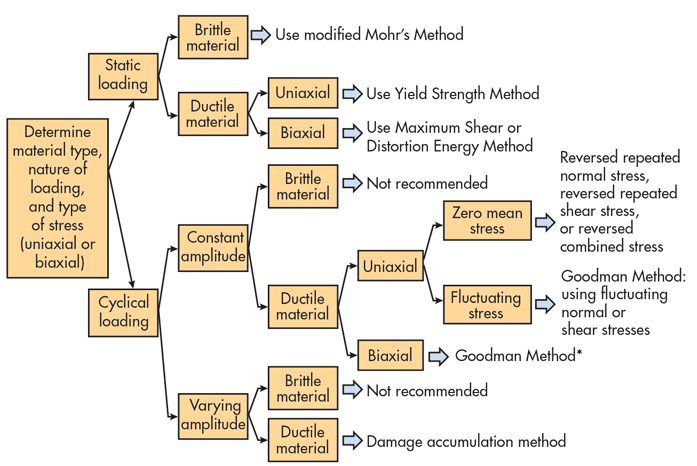
\includegraphics[width=0.9\textwidth]{tree.png}
	\caption{Example of a decision tree for choosing criteria.}
\end{figure}
\begin{multicols}{2}
	\section{USAGE OF COMPOSITES IN THE INDUSTRY}
	One of the biggest challenges to the design engineer in the aircraft and space industries is weight reduction. In these markets, each kilogram costs large amounts of money. In the sections above was explained how the sandwiched composites can reduce a significant amount of weight and conserve the sitiffness and strength that is needed in these applications. This is why they became one of the most efficient solutions to conjugate the highest bending stiffness and strength-to-weight ratios in structural components. Some of the applications of these composites are summarized in figure 8.

\end{multicols}

\begin{figure}[H]
	\centering
	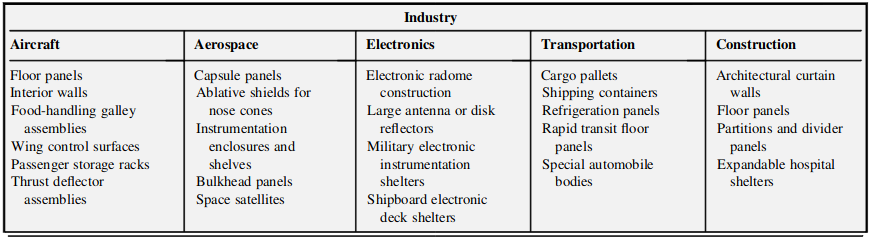
\includegraphics[width=\textwidth]{app.png}
	\caption{Table resuming the applications of composites by industry.}
\end{figure}
\begin{multicols}{2}
	Sandwiched composites are used not only in airplanes, but also in satellites and the naval industry. In satellites the solar panels are made from carbon---epoxy prepregs as skins, aluminum honeycomb and a film adhesive. Antenna reflectos are made from aramid---epoxy and carbon---cyanate prepegs in the skins and aramid---aluminum honeycomb. (See figure 9)
	\begin{figure}[H]
		\centering
		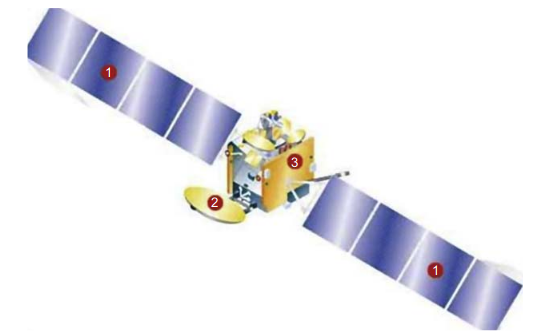
\includegraphics[width=0.5\textwidth]{sat.png}
		\caption{Composites applied in satellites.}
	\end{figure}
	In the aeronautical industry, as we can see in figure 10, shows the different materials used in an airplane.\supercite{sohel16} Today, for heavier-than-air machines there are three main types of composites in use: carbon fibre, glass and aramid --- reinforced epoxy. The latest development in the field of aerospace materials arise from the use of application-specific materials. For example, the Airbus A380, which at 61\% has the lowest percentage of aluminum by weight of all flying Airbus models, has 20 different alloys and tempers compared to the 6 utilised on the A320/330 aircraft. This lets the designers save up to 15 tonnes in weight, giving them the possibility of having a more optimal and efficient fuel system.\supercite{mrazova13}
	As a sidenote, the concern in use of composite materials arises mainly due to demands of high degree of reliability and safety of aerospace structures as against the complexity of composite behaviour and consequent difficulties in building prediction models. This creates and excesive reliance on testing at all stages; design and development, proving certification, and in-service inspection and repairs.\supercite{nayak14}

	\begin{figure}[H]
		\centering
		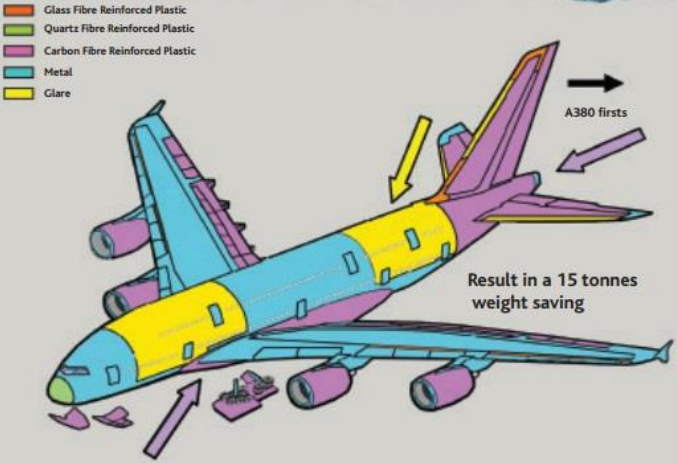
\includegraphics[width=0.5\textwidth]{acomp.png}
		\caption{The A380 material composition.}
	\end{figure}
	\section{THE FUTURE OF COMPOSITES}
	Ultimately we now live in a world which has a lot of restrictions and a lot of possibilities. The technological advances made in the last couple of decades are making their way into the more practical side of science. These not only make the way into more fuel efficient aircraft, but also more enviromentally friendly. New composite materials can be defined as materials which have yet to be applied in an "as-designed" application in aviation or any other industry. For the sake of example, ceramic matrix composites (CMCs) are excellent materials when it comes to their thermal properties. The possible applications of CMCs in aviation are generally in the hot section of the aero engines and include turbine disks, combustor linear, and turbine aerofoils.\supercite{nayak14}

	Other materials which have been expected are carbon nanotubes. These have been seen as having applications for electronics and shielding of large scale aircraft.

	What we may be able to conclude from this document is that composites are one of the most important parts of any modern aircraft. The provide high reliability and the mixed properties of many different materials. When it comes to the next generation of composite materials, clearly the possibilities are huge.
\end{multicols}
%%%%% Bib
\renewcommand\refname{REFERENCES}
\printbibliography

\end{document}
